%!TEX root = Slic3r-Manual.tex

\section{Extrudeuse Multiples} % (fold)
\label{sec:multiple_extruders}
\index{extruders!multiple}
\index{extrudeuse!multiple}

Une imprimante avec plus d'une extrudeuse peut être utilisé de différentes manières: L'extrudeuse supplémentaire pourrait imprimer une couleur ou une matière différente, ou pourrait être attribué à l'impression de caractéristiques particulières, telles que le remplissage, le support ou les périmètres.

L'impression multi-matières nécessite un objet conçu de manière appropriée généralement écrits au format AMF qui peut gérer plusieurs matériaux (voir les modèle de format au §\ref{sub:model_formats}).  Les détails sur la façon de créer de tel fichier sont donnés ci-dessous.


\subsection{Configurer les Extrudeuses} % (fold)
\label{sub:configuring_extruders}
\index{Printer Settings!General!Capabilities!Extruders}
\index{Paramètres de l'Imprimante!Fonctionnalités!Extrudeuses}

Dans l'onglet \texttt{Printer Settings} (Paramètres de l'Imprimante) il y a le paramètre \texttt{Extruders} (Extrudeuses), dans la section \texttt{Capabilities} (Fonctionnalités), ce qui permet de définir le nombre d'extrudeuses. Incrémenter cette valeur ajouter dynamiquement une autre définition d'extrudeuse dans le volet de gauche.

\begin{figure}[H]
\centering
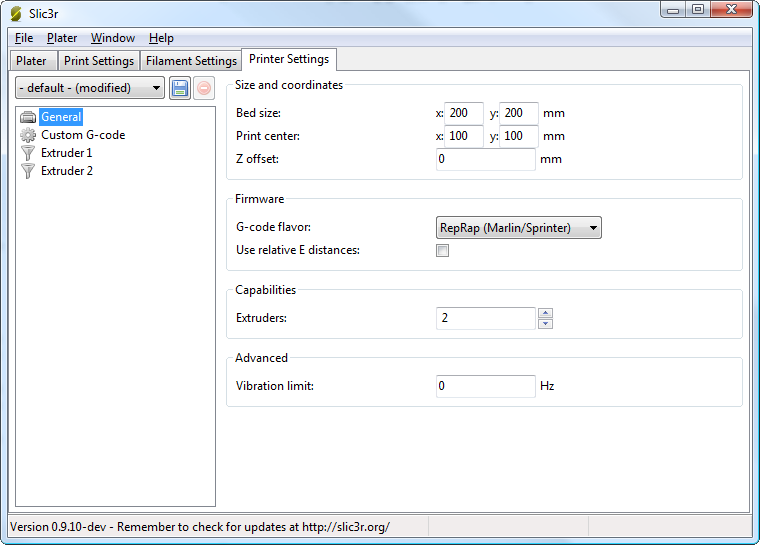
\includegraphics[keepaspectratio=true,width=1\textwidth]{expertmode/multipleextruders/printer_settings_general_multiple_extruder_options.png}
\caption{Paramètres d'Extrudeuses Multiples - Onglet Paramètre de l'Imprimante (Général).  Notez les deux extrudeuses définies dans le volet de gauche.}
\label{fig:printer_settings_general_multiple_extruder_options}
\end{figure}

Chaque extrudeuse peut être configuré comme d'habitude, mais il ya d'autres paramètres qui doivent être définis qui sont notamment les configurations multi-extrudeuse.

\begin{figure}[H]
\centering
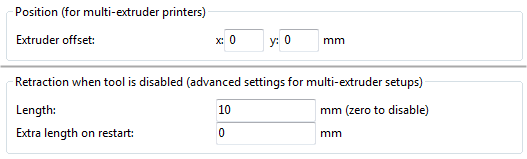
\includegraphics[keepaspectratio=true,width=1\textwidth]{expertmode/multipleextruders/printer_settings_extruder_multiple_extruder_options.png}
\caption{Paramètres d'Extrudeuses Multiples - Onglet Paramètre de l'Imprimante (Extruder).}
\label{fig:printer_settings_extruder_multiple_extruder_options}
\end{figure}

\index{Printer Settings!Extruder!Extruder offset}
\index{Paramètres de l'Imprimante!Décalage de l'extrudeuse}

l'\texttt{Extruder offset} (Décalage de l'extrudeuse) doit être utilisé si le microprogramme ne gère pas le décalage de chaque buse supplémentaire. La documentation de votre micrologiciel devrait vous dire si c'est le cas. Chaque extrudeuse supplémentaire a un décalage par rapport à la première. Si le firmware le gère , toutes les compensations peuvent rester à 0,0.

\index{Printer Settings!Extruder!Retraction!Length}
\index{Paramètres de l'Imprimante!Extrudeuse!Rétractation!Longueur}
Parce que l'extrudeuse secondaire sera en sommeil tandis que la première est cours d'utilisation, et vice-versa, il est important que le matériau soit suffisamment rétractée pour cesser le suintement.  Comme avec les réglages ordinaires de rétractation (voir p. \pageref{fig:retraction_settings}) le paramètre \texttt{Length} (Longueur) est mesurée à partir du filament entrant dans l'extrudeuse.

% subsection configuring_extruders (end)

\subsection{Attribution de filaments} % (fold)
\label{sub:assigning_filaments}
\index{Plater}
\index{Surface de Travail}
Quand un profil d'imprimante avec plusieurs extrudeuses a été sélectionné, l'onglet \texttt{Plater} (Surface de Travail) permet la sélection d'un filament différent pour chaque extrudeuse.

\begin{figure}[H]
\centering
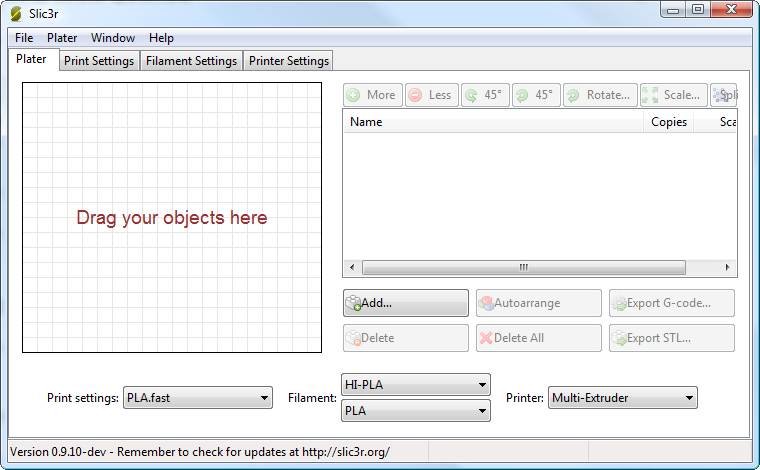
\includegraphics[keepaspectratio=true,width=1\textwidth]{expertmode/multipleextruders/plater_multi_filament.png}
\caption{Surface de travail avec de multiple paramètre de filaments.}
\label{fig:plater_multi_filament}
\end{figure}

% subsection assigning_filaments (end)

\subsection{Affectation des extrudeuses pour les objets mono-matière} % (fold)
\label{sub:assigning_extruders}
\index{Print Settings!Multiple Extruders}
\index{Paramètres de l'Imprimante!Extrudeuse Multiple}

Pour les impressions de matériaux unique, où l'extrudeuse secondaire a pour mission une extrusion particuliere, la section \texttt{Multiple Extruders} (Extrudeuses multiples) de l'onglet \texttt{Print Settings} (Paramètres de l'imprimante) donne la possibilité d'assigner une extrudeuse pour chaque type d'extrusion.

\begin{figure}[H]
\centering
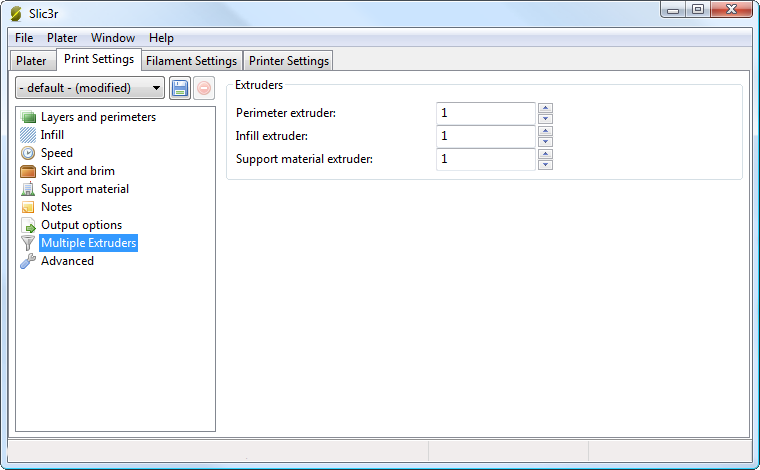
\includegraphics[keepaspectratio=true,width=1\textwidth]{expertmode/multipleextruders/print_settings_multiple_extruder_options.png}
\caption{Paramètres d'Extrudeuse Multiple - Onglet Paramètre d'Impression.}
\label{fig:advanced_multiple_extruder_options}
\end{figure}

% subsection assigning_extruders (end)

\subsection{Configurer le Changement d'Outil} % (fold)
\label{sub:configuring_tool_changes}

\index{Printer Settings!Custom G-code!Tool change G-code}
\index{Paramètres de l'Imprimante!G-code personalisé!G-code de changement d'outil}

La section \texttt{Custom G-code} (G-code personalisé) de l'onglet \texttt{Printer Settings} (Paramètres de l'Imprimante) dispose d'une option d'insertion de G-code entre les changements d'outils. Comme avec toutes les sections personnalisé G-code, les variables d'environement peuvent être utilisées afin de référencer les paramètres Slic3r.  Cela inclus les variables [previous\_extruder] et [next\_extruder].

\begin{figure}[H]
\centering
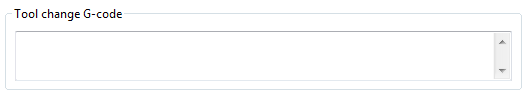
\includegraphics[keepaspectratio=true,width=1\textwidth]{expertmode/multipleextruders/printer_settings_custom_gcode.png}
\caption{Paramètres d'Extrudeuse Multiple - G-code de Changement d'outil.}
\label{fig:printer_settings_custom_gcode}
\end{figure}

% subsection configuring_tool_changes (end)


\subsection{Impression d'objets multi-matières} % (fold)
\label{sub:printing_multi_material_objects}

Si un fichier multi-matériaux AMF existe déjà, parce que le programme de CAO peut exporter un tel format, alors celui-ci peut être chargé dans Slic3r de façon habituelle. Le mappage entre matières de l'objet et les extrudeuses est séquentielle, c'est à dire que la premiere matière est affecté à la première extrudeuse, etc.

% subsection printing_multi_material_objects (end)


\subsection{Génération de fichiers AMF multi-matière} % (fold)
\label{sub:generating_multi_material_amf_files}

Slic3r a la capacité de combiner plusieurs fichiers STL dans un fichier multi-matière AMF.

\index{Menu!Combine multi-material STL files...}
\index{Menu!Combiner des fichiers STL multi-matière...}

\begin{itemize}
    \item Diviser la conception originale dans les différentes parties au sein du programme de CAO, et exporter chaque partie en STL.
    \item Dans Slic3r, choisissez \texttt{Combine multi-material STL files...} (Combiner des fichiers STL multi-matière...) a partir du menu \texttt{File} (Fichier).
    \item Lorsque vous êtes invité avec une boîte de dialogueChoisissez le premier STL, qui sera attribué à la première matière (et donc la première extrudeuse). Cliquez sur \texttt{Open} pour être invité au prochain STL, et ainsi de suite jusqu'à ce que chaque STL soit affectés à une matière. Pour signaler qu'il n'y a plus de fichiers STL, choisissez \texttt{Cancel} (Annuler).
    \item La boîte de dialogue suivante demande l'emplacement et le nom du fichier de l'AMF.
\end{itemize}

Une fois généré le fichier peut être chargé et imprimé comme décrit ci-dessus.

% subsection generating_multi_material_amf_files (end)

% section multipe_extruders (end)